\chapter{PLAYER CHARACTER CLASSES}

\begin{multicols}{2}

All player characters are members of a specific class.  Their class embodies their special training before they became an adventurer.  \index{Class Groups}There are four class groups; warrior, wizard, priest, and rogue.  Each group bestows the same hit dice progression, attack bonus, and saving throw progression.

\section{ABILITY SCORE REQUIREMENTS}

All classes require a \index{Ability Scores!Class Requirements}minimum ability score to qualify for them.  If a character does not qualify for any class the GM should allow the player to re-roll their ability scores or increase a score to match a minimum.

\noindent
\begin{minipage}{\columnwidth}

\captionof{table}{Class Ability Score Requirements}\label{classreqs}
\noindent
\begin{tabular}{|p{0.206\columnwidth}|m{0.074\columnwidth}|m{0.074\columnwidth}|m{0.074\columnwidth}|m{0.074\columnwidth}|m{0.074\columnwidth}|m{0.074\columnwidth}|}
\hline
Character Class		& Str	& Dex	& Con	& Int	& Wis	& Cha \\
\hline\hline
\rowcolor[gray]{.9}Fighter				& 9		& --	& --	& --	& --	& -- \\
Paladin				& 12	& --	& 9		& --	& 13	& 17 \\
\rowcolor[gray]{.9}Ranger				& 13	& 13	& 14	& --	& 14	& -- \\
Mage				& --	& --	& --	& 9		& --	& -- \\
\rowcolor[gray]{.9}Specialist Mage*	& Var	& Var	& Var	& Var	& Var	& Var \\
Cleric				& --	& --	& --	& --	& 9		& -- \\
\rowcolor[gray]{.9}Druid				& --	& --	& --	& --	& 12	& 15 \\
Thief				& --	& 9		& --	& --	& --	& -- \\
\rowcolor[gray]{.9}Bard				& --	& 12	& --	& 13	& --	& 15 \\
\hline
\end{tabular}
\noindent
\begin{tabular}{p{\columnwidth}}
*Specialist mage ability score requirements vary \\
\end{tabular}\vspace{.5em}

\end{minipage}

\section{CLASS DESCRIPTIONS}

Each class group includes a basic description followed by their defining features and abilities.  A table lists their hit dice, combat rating, and saving throws followed by any other special abilities directly related to the class in question.  After a certain level a class stops gaining hit dice and constitution bonuses to hit dice.  From then on they receive a fixed rate of hit points.  

Each individual class lists the racial, ability, and alignment restrictions.  \index{Prime Requisite}Characters who meet their prime requisite receive a +10\% bonus to earned experience points.  Weapons and armor list the restrictions the class has for equipment. 

 
\index{Warriors}\section{WARRIOR}

Warriors are combatants that rely on strength, weapons training, and tactics to dominate the battlefield.  Warriors charge into battle with sword and shield or fire accurate shots from the sidelines.  

\noindent
\includegraphics[width=\columnwidth, height=1.75in]{testblock.pdf}  

\end{multicols}

%\newpage

\noindent
\begin{minipage}{\columnwidth}

\captionof{table}{Warrior Advancement}\label{warrioradvancement}
\noindent
\begin{tabular}{|m{0.176\columnwidth}|m{0.176\columnwidth}|m{0.176\columnwidth}|m{0.176\columnwidth}|m{0.176\columnwidth}|}
\hline
Level	& Fighter	& Paladin/ Ranger	& Hit Dice (d10)	& THACO \\
\hline\hline
\rowcolor[gray]{.9}1		& 0			& 0			& 1		& 20 \\
2		& 2,000		& 2,250		& 2		& 19 \\
\rowcolor[gray]{.9}3		& 4,000		& 4,500		& 3		& 18 \\
4		& 8,000		& 9,000		& 4		& 17 \\
\rowcolor[gray]{.9}5		& 16,000	& 18,000	& 5		& 16 \\
6		& 32,000	& 36,000	& 6		& 15 \\
\rowcolor[gray]{.9}7		& 64,000	& 75,000	& 7		& 14 \\
8		& 125,000	& 150,000	& 8		& 13 \\
\rowcolor[gray]{.9}9		& 250,000	& 300,000	& 9		& 12 \\
10		& 500,000	& 600,000	& 9~+~3	& 11 \\
\rowcolor[gray]{.9}11		& 750,000	& 900,000	& 9~+~6	& 10 \\
12		& 1,000,000	& 1,200,000	& 9~+~9	& 9 \\
\rowcolor[gray]{.9}13		& 1,250,000	& 1,500,000	& 9~+~12	& 8 \\
14		& 1,500,000	& 1,800,000	& 9~+~15	& 7 \\
\rowcolor[gray]{.9}15		& 1,750,000	& 2,100,000	& 9~+~18	& 6 \\
16		& 2,000,000	& 2,400,000	& 9~+~21	& 5 \\
\rowcolor[gray]{.9}17		& 2,250,000	& 2,700,000	& 9~+~24	& 4 \\
18		& 2,500,000	& 3,000,000	& 9~+~27	& 3 \\
\rowcolor[gray]{.9}19		& 2,750,000	& 3,300,000	& 9~+~30	& 2 \\
20		& 3,000,000	& 3,600,000	& 9~+~33	& 1 \\
\hline
\end{tabular}

\end{minipage}

\noindent
\begin{minipage}{\columnwidth}

\captionof{table}{Warrior Saving Throws}\label{warriorsaves}
\noindent
\begin{tabular}{|m{0.12\columnwidth}|m{0.148\columnwidth}|m{0.148\columnwidth}|m{0.148\columnwidth}|m{0.148\columnwidth}|m{0.148\columnwidth}|}
\hline
Level	& Paralyzation, Poison, or Death	& Rod, Staff, or Wand	& Petrification or Polymorph	& Breath Weapon	& Spell \\
\hline\hline
\rowcolor[gray]{.9}1--2		& 14	& 16	& 15	& 17	& 17 \\
3--4		& 13	& 15	& 14	& 16	& 16 \\
\rowcolor[gray]{.9}5--6		& 11	& 13	& 12	& 13	& 14 \\
7--8		& 10	& 12	& 11	& 12	& 13 \\
\rowcolor[gray]{.9}9--10	& 8		& 10	& 9		& 9		& 11 \\
11--12	& 7		& 9		& 8		& 8		& 10 \\
\rowcolor[gray]{.9}13--14	& 5		& 7		& 6		& 5		& 8 \\
15--16	& 4		& 6		& 5		& 4		& 7 \\
\rowcolor[gray]{.9}17+		& 3		& 5		& 4		& 4		& 6 \\
\hline
\end{tabular}

\end{minipage}

\begin{multicols}{2}

\noindent
\begin{minipage}{\columnwidth}

\captionof{table}{Warrior Attacks per Round}\label{warriorattacks}
\noindent
\begin{tabular}{|m{0.45\textwidth}|m{0.45\textwidth}|}
\hline
Warrior Level	& Attacks per Round \\
\hline\hline
\rowcolor[gray]{.9}1--6		& 1/round \\
7--12	& 3/2 rounds \\
\rowcolor[gray]{.9}13+		& 2/round \\
\hline
\end{tabular}

\end{minipage}

\subsection{FIGHTER}

\index{Fighters}Fighters are men-at-arms and experts at weapon combat.  They're the frontlines of every battle, the archers that soften targets from afar, the charging cavalry, and with a little luck, skill in arms, and a lot of determination, they eventually become warrior-lords that lead entire armies.

\paragraph{Ability Requirements:} Str 9

\paragraph{Race:} Any

\paragraph{Prime Requisite:} Str 16+

\paragraph{Alignment:} Any

\paragraph{Weapons:} All

\paragraph{Armor:} All + shields

\index{Combat Skill Aptitude!Fighters}\paragraph{Combat Skill Aptitude:} When choosing combat skills, a single class fighter is at a distinct advantage over all others.  They alone are able to specialize with specific weapons and unarmed combat methods, as well as become skilled in more than one combat method (Refer to Combat Skills).

\index{Lordship!Fighters}\paragraph{Lord:} At 9\textsuperscript{th} level, a fighter becomes a ``Lord" or gains some other special title.  A lord's reputation is enough that they're entitled to land or the right to build a stronghold.  With a stronghold, a lord attracts a small army of men-at-arms as well as an elite guard that enforce his rule.  While the loyalty of these troops is greater than the average hireling, the lord is still expected to pay their wages and treat them fairly.  

The GM is in charge of assigning the lord's men.  A good rule of thumb is one leader half the lord's level, eighty 0-level soldiers (pike men, archers, and mace men), and an elite guard of twelve 1\textsuperscript{st} level knights.   

 
\subsection{PALADIN}

\index{Paladins}Paladins are the quintessential knights-in-shining-armor.  They're noble warriors of unwavering good who protect the innocent, crusade against evil, and uphold the law while challenging those who abuse the rules for their own benefit.  Because of their strict code of conduct, few achieve paladin-hood and fewer still walk the path their whole lives without falling.

\paragraph{Ability Requirements:} Str 12, Con 9, Wis 13, and Cha 17

\paragraph{Race:} Human

\paragraph{Prime Requisite:} Str and Cha 16+

\paragraph{Alignment:} Lawful Good

\paragraph{Weapons:} All

\paragraph{Armor:} All + shields

\index{Detect Evil!Paladins}\paragraph{Detect Evil:} Paladins can cast a \textit{detect evil} with a 60' range by concentrating for 1 round.  They can only detect evil monsters and characters, not magic.

\index{Divine Grace!Paladins}\paragraph{Divine Grace:} Paladins receive a +2 bonus on all saving throws.

\index{Divine Health!Paladins}\paragraph{Divine Health:} Paladins are immune to all diseases but not curses such as lycanthropy.
  
\index{Lay on Hands!Paladins}\paragraph{Lay on Hands:} Paladins can heal by the laying on of hands.  1/day, a paladin can heal 2 HP per experience level on himself or someone else.  

\index{Cure Disease!Paladins}\paragraph{Cure Disease:} Paladins can cast \textit{cure disease} once per week per 5 experience levels.

\index{Aura of Protection!Paladins}\paragraph{Aura of Protection:} Paladins emit an aura of protection in a 10' radius.  All summoned and evil creatures suffer a $-1$ penalty to attack rolls within the aura.

\index{Circle of Power!Paladins}\paragraph{Circle of Power:} A paladin wielding a holy sword projects power in a 15' radius when the sword is unsheathed and wielded.  This ability dispels enemy magic up to the experience level of the paladin.

\index{Turn Undead!Paladins}\paragraph{Turn Undead:} A paladin can turn undead, devils, and demons at 3\textsuperscript{rd} level as if he were a 1\textsuperscript{st} level cleric.  The paladin's turning level increases to 2\textsuperscript{nd} at 4\textsuperscript{th} level, 3\textsuperscript{rd} at 5\textsuperscript{th}, etc.

\index{Special Mount!Paladins}\paragraph{Special Mount:} A paladin gains a special mount at 4\textsuperscript{th} level.  The paladin's mount appears as fast as possible when called.  It is then magically bound and always loyal to the paladin.  The paladin can communicate simple commands to his mount without fail.  The GM should determine the nature of the paladin's mount and the mount should be obtained as part of an adventure.

\index{Priest Spells!Paladins}\paragraph{Priest Spells:} Paladins can cast priest spells beginning at 9\textsuperscript{th} level.  He can only cast spells in the Combat, Divination, Healing, and Protection spheres.  Paladins do not gain bonus spells for high wisdom.  Paladins cannot cast cleric or druid spells from scrolls nor use priest items unless also allowed to warriors.

\noindent
\begin{minipage}{\columnwidth}

\captionof{table}{Priest Spells per Level}\label{paladinspells}
\noindent
\begin{tabular}{|m{0.181\columnwidth}|m{0.181\columnwidth}|m{0.084\columnwidth}|m{0.085\columnwidth}|m{0.084\columnwidth}|m{0.085\columnwidth}|}
\hline
Paladin Level	& Caster Level	& 1	& 2	& 3	& 4 \\
\hline\hline
\rowcolor[gray]{.9}9	& 1	 	& 1	& --	& --	& -- \\
10	& 2	 	& 2	& --	& --	& -- \\
\rowcolor[gray]{.9}11	& 3	 	& 2	& 1		& --	& -- \\
12	& 4	 	& 2	& 2		& --	& -- \\
\rowcolor[gray]{.9}13	& 5	 	& 2	& 2		& 1		& -- \\
14	& 6	 	& 3	& 2		& 1		& -- \\
\rowcolor[gray]{.9}15	& 7	 	& 3	& 2		& 1		& 1 \\
16	& 8		& 3	& 3		& 2		& 1 \\
\rowcolor[gray]{.9}17	& 9*	& 3	& 3		& 3		& 1 \\
18	& 9		& 3	& 3		& 3		& 1 \\
\rowcolor[gray]{.9}19	& 9		& 3	& 3		& 3		& 2 \\
20	& 9		& 3	& 3		& 3		& 3 \\
\hline
\end{tabular}
\noindent
\begin{tabular}{p{\columnwidth}}
*Maximum caster level for a paladin \\
\end{tabular}\vspace{.5em}

\end{minipage}

\index{Code of Conduct!Paladins}\paragraph{The Paladin's Code of Conduct:}

\begin{itemize}

\item Paladins are lawful good.  If a paladin knowingly commits a chaotic act, he must confess as soon as possible to a 7\textsuperscript{th} level or higher priest and seek penance.  If a paladin knowingly and willfully commits an evil act, his status and powers are stripped permanently.  A fallen paladin becomes a fighter of the same level, losing any excess experience points he may have.  A paladin that commits an evil act against his will (through magic or possession) loses his status and functions as a fighter of the same experience point value until he atones for his deed.

\item Paladins are humble.  They may not carry more than 10 magical items, restricted to one suit of armor, one shield, four weapons (ammunition does not count), and four miscellaneous items.  Paladins can haul and transport magical items such as in saddlebags or a cart, but as an act of humility they cannot have on their person more than their restriction.  If a paladin encounters an opponent while carrying magical items that exceed his limit, he must drop them before fighting.

\item Paladins are charitable.  Paladins must tithe at least 10\% of their total income to a charitable or lawful good organization every month. They may only keep enough treasure to modestly support themselves, pay servitors a reasonable rate, and maintain a stronghold, although a fraction of the funds may be set aside for construction, repair, and emergencies.  All excess wealth must be donated to a charitable cause (usually the paladin's church) and may never be given to PCs or NPCs.

\item Paladins are righteous.  Paladins only employ lawful good henchmen or those who act in a noble manner.  Paladins tolerate characters of any alignment so long as they do no evil in their presences; however, paladins try to convert non-good followers by setting good examples and through virtuous actions.  

\end{itemize}

\subsection{RANGER}

\index{Rangers}Rangers are warriors, hunters of evil, protectors of nature, and defenders of mankind from the nastier parts of nature.  Rangers scout their area for encroaching armies, track criminals, protect the land from evil interlopers, and lead small bands against strong resistance.  Although rangers have the same abilities as fighters, they prefer to wear light armor and assault enemies from afar or from the shadows before closing in.

\paragraph{Ability Requirements:} Str 13, Dex 13, Con 14, and Wis 14

\paragraph{Race:} Human, Elf, or Half-elf

\paragraph{Prime Requisite:} Str, Dex, and Wis 16+

\paragraph{Alignment:} Lawful, neutral, or chaotic good.

\paragraph{Weapons:} All

\paragraph{Armor:} All + shields

\index{Tracking!Rangers}\paragraph{Tracking:} Rangers are expert trackers.  To track a creature, the ranger rolls a 1d20 against his wisdom score.  If the result is equal to or lower than his ability score, the ranger successfully follows the trail.  Cumulative modifiers may apply to the ranger's wisdom score, further modifying his chance at success.  If the modifiers reduce the tracker's wisdom score to 0, the trail is impossible to follow.

\noindent
\begin{minipage}{\columnwidth}

\captionof{table}{Ranger Tracking Modifiers}\label{trackingmods}
\noindent
\begin{tabular}{|m{0.72\columnwidth}|m{0.18\columnwidth}|}
\hline
Terrain	& Modifier \\
\hline\hline
\rowcolor[gray]{.9}Soft or muddy ground	& +4 \\
Thick brush or vines	& +3 \\
\rowcolor[gray]{.9}Obvious signs of passage (muddy footprints, dust, etc.)	& +2 \\
Hard earth, wood floor	& 0 \\
\rowcolor[gray]{.9}Rocky ground or shallow water	& $-10$ \\
Every two creatures in group	& +1 \\
\rowcolor[gray]{.9}Every 12 hours since trail was made	& $-1$ \\
Every hour of rain or snow	& $-5$ \\
\rowcolor[gray]{.9}Moonlight or candlelight	& $-6$ \\
Tracked party hides trail	& $-5$ \\
\hline
\end{tabular}

\end{minipage}

In order to track a creature, there must be evidence of a trail or witnesses to point the way.  Additional checks are made under specific circumstances:

\begin{itemize}

\item The trail becomes more difficult to track (splitting direction, difficult terrain, environmental hazards)

\item Tracks of a similar nature cross the trail.

\item Resume tracking after a rest.

\end{itemize}

If the tracker fails, he may retry after an hour of searching.  If the second roll fails the trail is lost.  If multiple trackers are present, each additional tracker adds +1 to the wisdom score of the most expert tracker.  If the expert tracker loses the trail, it is lost for all trackers aiding him. 

Every time the tracker rolls a check, he may roll a second check to determine the type of creatures and an approximation of their numbers as determined by the GM.

\index{Expert Tracking!Rangers}\paragraph{Expert Tracking:} Every third level, a ranger receives a +1 bonus to his tracking (+1 at 3\textsuperscript{rd}, +2 at 6\textsuperscript{th}, etc.).  

\index{Hide in Shadow!Rangers}\index{Move Stealthily!Rangers}\index{Ranger Abilities}\paragraph{Ranger Abilities:} Rangers are experts at stealth and can hide and move stealthily.  These abilities are modified by dexterity and race, but not armor, and otherwise function exactly like thieving skills of the same name.  Rangers cannot hide or move stealthily in armor heavier than studded leather.  When attempting these skills in artificial settings (city streets, inside buildings, crypts), his chance of success is halved. 

\noindent
\begin{minipage}{\columnwidth}

\captionof{table}{Ranger Abilities}\label{rangerabilities}
\noindent
\begin{tabular}{|m{0.123\columnwidth}|m{0.147\columnwidth}|m{0.147\columnwidth}|m{.098\columnwidth}|m{.049\columnwidth}|m{.049\columnwidth}|m{.049\columnwidth}|}
\hline
 & & & & \multicolumn{3}{c|}{Spells}\\
Ranger Level	& Hide in Shadow*	& Move Stealth\-ily*	& Caster Level	& 1	& 2	& 3 \\
\hline\hline
\rowcolor[gray]{.9}1	& 10\%	& 15\%	& --	& --	& --	& -- \\
2	& 15\%	& 21\%	& --	& --	& --	& -- \\
\rowcolor[gray]{.9}3	& 20\%	& 27\%	& --	& --	& --	& -- \\
4	& 25\%	& 33\%	& --	& --	& --	& -- \\
\rowcolor[gray]{.9}5	& 31\%	& 40\%	& --	& --	& --	& -- \\
6	& 37\%	& 47\%	& --	& --	& --	& -- \\
\rowcolor[gray]{.9}7	& 43\%	& 55\%	& --	& --	& --	& -- \\
8	& 49\%	& 62\%	& 1	& 1	& --	& -- \\
\rowcolor[gray]{.9}9	& 56\%	& 70\%	& 2	& 2	& --	& -- \\
10	& 63\%	& 78\%	& 3	& 2	& 1	& -- \\
\rowcolor[gray]{.9}11	& 70\%	& 86\%	& 4	& 2	& 2	& -- \\
12	& 77\%	& 94\%	& 5	& 2	& 2	& 1 \\
\rowcolor[gray]{.9}13	& 85\%	& 99\%	& 6	& 3	& 2	& 1 \\
14	& 93\%	& 99\%	& 7	& 3	& 2	& 2 \\
\rowcolor[gray]{.9}15	& 99\%	& 99\%	& 8	& 3	& 2	& 2 \\
16	& 99\%	& 99\%	& 9	& 3	& 3	& 3 \\
\hline
\end{tabular}
\noindent
\begin{tabular}{p{.95\columnwidth}}
*See thief's description for abilities. Abilities modified by race and dexterity as a thief. \\
\end{tabular}\vspace{.5em}

\end{minipage}

\index{Two-weapon Method!Rangers}\paragraph{Two Weapon Style:} Rangers can fight with two weapons without penalty, as long as they are wearing studded leather or lighter armors (Refer to Two Weapon Fighting and also Two-Weapon Combat Method).

\index{Favored Enemy!Rangers}\paragraph{Favored Enemy:} At any point before 2\textsuperscript{nd} level, rangers choose a species of creature that represents their chosen enemy.  Typical creatures include those native to the ranger's homeland and are found in natural settings, such as giants, gnolls, goblins, and undead (GM has final say).  The ranger gains a +4 bonus to attack rolls against his favored enemy.  His hatred is hard to mask resulting in a -4 penalty to reaction rolls against the favored enemy.  The ranger will always attack his favored enemy first in combat unless another creature presents a greater threat.

\index{Animal Empathy!Rangers}\paragraph{Animal Empathy:} Rangers can calm and befriend domesticated animals instantly.  Wild animals must roll a saving throw vs. rods to resist a ranger's effect.  The ranger imposes a $-1$ penalty to this saving throw and an additional $-1$ for every 3 levels (-2 at 3\textsuperscript{rd}, $-3$ at 6\textsuperscript{th}, etc.).  If the animal fails, the ranger can shift its reaction one category as he chooses.  

\index{Priest Spells!Rangers}\paragraph{Priest Spells:} Rangers learn priest spells related to the Plant and Animal spheres at 8\textsuperscript{th} level.  Rangers do not gain bonus spells for high wisdom.  The ranger's spells otherwise function exactly like a priest's.  Spell progression is shown on the table above.

\index{Followers!Rangers}\paragraph{Followers:} At 10\textsuperscript{th} level, rangers attract followers of the GM's choice.  These followers tend to be experienced woodsmen, trackers, and semi-intelligent or magical animals appropriate to the terrain.  As a guideline, no more than a dozen followers seek out a particular ranger.

\index{Code of Conduct!Rangers}\paragraph{The Ranger's Code of Conduct:}

\begin{itemize}

\item Rangers are Good: Rangers must always remain good.  A ranger who willingly commits an evil act irrevocably loses his status and becomes a fighter of the same level, losing any excess experience points.  A ranger who unwillingly commits an evil act, through magic or otherwise, cannot gain experience points until he atones through good deeds.  These deeds are determined by the GM and could involve challenging an evil lord, freeing captives from an evil master, or slaying a powerful evil beast.  

\item Rangers are Loners: Rangers can never have henchmen, hirelings, or servants at any time, although they may travel and associate with fellow adventurers.  This restriction is lifted after 8\textsuperscript{th} level.  

\item Rangers are Frugal: Rangers cannot own more treasure than they can carry.  Excess treasure must either be converted to portable form (gems, art, bank notes) or donated to a good NPC-run charitable organization.  

\end{itemize}
 
\index{Wizards}\section{WIZARD}

Wizards are men and women who study the arcane forces of the universe and gain mastery over it.  Wizards pour over dusty tomes and scour ancient ruins for knowledge and lore.  They memorize words of power, imprinting them into their brains, and utter their phrases to cast powerful magic.  Wizards who study all the known schools of magic are called mages.  Some wizards forgo study of certain schools in order to gain a greater mastery over another sacrificing versatility for strength.  These wizards are called by their specialization; a master of illusion is an illusionist and so forth.

\index{Spell Book!Wizards}All wizards begin with a free 100-page spell book.  \index{Starting Spells!Wizards}Beginning wizards know 3d4 level 1 spells, two of which must be \textit{read magic} and \textit{detect magic}, and the other spells of the player's choice.  \index{Gaining Spells!Wizards}Whenever a wizard gains enough levels of experience to cast the next level of spells, they freely add 1 spell of the new spell level to their book.

\index{Preparing Spells!Wizards}Wizards prepare spells by studying their spell book.  Each spell slot per level allows them to memorize one spell.  Wizards can memorize multiple castings of the same spell but are still restricted by the number of spell slots per level they can memorize.  Once a spell is cast, the slot is spent and the wizard must study his spell book again to rememorize it.  Spell slots are not interchangeable; a level 1 spell cannot be stored in a level 2 slot and vice versa.

\noindent
\begin{minipage}{\columnwidth}

\captionof{table}{Wizard Advancement}\label{wizardadvancement}
\noindent
\begin{tabular}{|m{0.185\columnwidth}|m{0.185\columnwidth}|m{0.245\columnwidth}|m{0.185\columnwidth}|}
\hline
Level	& Mage/ Specialist	& Hit Dice (d4)	& THACO \\
\hline\hline
\rowcolor[gray]{.9}1	& 0				& 1		& 20 \\
2	& 2,500			& 2		& 20 \\
\rowcolor[gray]{.9}3	& 5,000			& 3		& 20 \\
4	& 10,000		& 4		& 19 \\
\rowcolor[gray]{.9}5	& 20,000		& 5		& 19 \\
6	& 40,000		& 6		& 19 \\
\rowcolor[gray]{.9}7	& 60,000		& 7		& 18 \\
8	& 90,000		& 8		& 18 \\
\rowcolor[gray]{.9}9	& 135,000		& 9		& 18 \\
10	& 250,000		& 10	& 17 \\
\rowcolor[gray]{.9}11	& 375,000		& 10~+~1	& 17 \\
12	& 750,000		& 10~+~2	& 17 \\
\rowcolor[gray]{.9}13	& 1,125,000		& 10~+~3	& 16 \\
14	& 1,500,000		& 10~+~4	& 16 \\
\rowcolor[gray]{.9}15	& 1,875,000		& 10~+~5	& 16 \\
16	& 2,250,000		& 10~+~6	& 15 \\
\rowcolor[gray]{.9}17	& 2,625,000		& 10~+~7	& 15 \\
18	& 3,000,000		& 10~+~8	& 15 \\
\rowcolor[gray]{.9}19	& 3,375,000		& 10~+~9	& 14 \\
20	& 3,750,000		& 10~+~10	& 14 \\
\hline
\end{tabular}

\end{minipage}

\end{multicols}

\noindent
\begin{minipage}{\columnwidth}

\captionof{table}{Wizard Spells per Level}\label{wizardspells}
\noindent
\begin{tabular}{|m{0.13\textwidth}|m{0.07\textwidth}|m{0.07\textwidth}|m{0.07\textwidth}|m{0.07\textwidth}|m{0.07\textwidth}|m{0.07\textwidth}|m{0.07\textwidth}|m{0.07\textwidth}|m{0.07\textwidth}|}
\hline
Wizard Level	& 1	& 2	& 3	& 4	& 5	& 6	& 7	& 8	& 9 \\
\hline\hline
\rowcolor[gray]{.9}1	& 1	& --	& --	& --	& --	& --	& --	& --	& -- \\
2	& 2	& --	& --	& --	& --	& --	& --	& --	& -- \\
\rowcolor[gray]{.9}3	& 2	& 1		& --	& --	& --	& --	& --	& --	& -- \\
4	& 3	& 2		& --	& --	& --	& --	& --	& --	& -- \\
\rowcolor[gray]{.9}5	& 4	& 2		& 1		& --	& --	& --	& --	& --	& -- \\
6	& 4	& 2		& 2		& --	& --	& --	& --	& --	& -- \\
\rowcolor[gray]{.9}7	& 4	& 3		& 2		& 1		& --	& --	& --	& --	& -- \\
8	& 4	& 3		& 3		& 2		& --	& --	& --	& --	& -- \\
\rowcolor[gray]{.9}9	& 4	& 3		& 3		& 2		& 1		& --	& --	& --	& -- \\
10	& 4	& 4		& 3		& 2		& 2		& --	& --	& --	& -- \\
\rowcolor[gray]{.9}11	& 4	& 4		& 4		& 3		& 3		& --	& --	& --	& -- \\
12	& 4	& 4		& 4		& 4		& 4		& 1		& --	& --	& -- \\
\rowcolor[gray]{.9}13	& 5	& 5		& 5		& 4		& 4 	& 2		& --	& --	& -- \\
14	& 5	& 5		& 5		& 4		& 4		& 2		& 1		& --	& -- \\
\rowcolor[gray]{.9}15	& 5	& 5		& 5		& 5		& 5		& 2		& 1		& --	& -- \\
16	& 5	& 5		& 5		& 5		& 5		& 3		& 2		& 1		& -- \\
\rowcolor[gray]{.9}17	& 5	& 5		& 5		& 5		& 5		& 3		& 3		& 2		& -- \\
18	& 5	& 5		& 5		& 5		& 5		& 3		& 3		& 2		& 1 \\
\rowcolor[gray]{.9}19	& 5	& 5		& 5		& 5		& 5		& 3		& 3		& 3		& 1 \\
20	& 5	& 5		& 5		& 5		& 5		& 4		& 3		& 3		& 2 \\
\hline
\end{tabular}

\end{minipage}

%\newpage

\noindent
\begin{minipage}{\columnwidth}

\captionof{table}{Wizard Saving Throws}\label{wizardsaves}
\noindent
\begin{tabular}{|m{0.12\columnwidth}|m{0.148\columnwidth}|m{0.148\columnwidth}|m{0.148\columnwidth}|m{0.148\columnwidth}|m{0.148\columnwidth}|}
\hline
Level	& Paralyzation, Poison, or Death	& Rod, Staff, or Wand	& Petrification or Polymorph	& Breath Weapon	& Spell \\
\hline\hline
\rowcolor[gray]{.9}1--5		& 14	& 11	& 13	& 15	& 12 \\
6--10	& 13	& 9		& 11	& 13	& 10 \\
\rowcolor[gray]{.9}11--15	& 11	& 7		& 9		& 11	& 8 \\
16--20	& 10	& 5		& 7		& 9		& 6 \\
\rowcolor[gray]{.9}21+		& 8		& 3		& 5		& 7		& 4 \\
\hline
\end{tabular}

\end{minipage}

\noindent
\begin{minipage}{\columnwidth}

\captionof{table}{Specialist Wizard Restrictions}\label{specialistrestrictions}
\noindent
\begin{tabular}{|p{0.12\textwidth}|p{0.20\textwidth}|p{0.09\textwidth}|p{0.49\textwidth}|}
\hline
Specialist	& Race	& Min Score	 & School(s) Allowed \\
\hline\hline
\rowcolor[gray]{.9}Abjurer	& Human	& 15 Wis	& Abjuration, Conjuration, Greater Divination, Enchantment, Evocation, Necromancy \\

Conjurer	& Human, Half-elf	& 15 Con	& Conjuration, Abjuration, Lesser Divination, Enchantment, Illusion, Necromancy, Transmutation \\

\rowcolor[gray]{.9}Diviner	& Human, Elf, Half-elf	& 16 Wis	& Greater Divination, Abjuration, Enchantment, Evocation, Illusion, Necromancy, Transmutation \\

Enchanter	& Human, Elf, Half-elf	& 16 Cha	& Enchantment, Abjuration, Conjuration, Greater Divination, Illusion, Transmutation \\

\rowcolor[gray]{.9}Illusionist	& Human, Gnome	& 16 Dex	& Illusion, Conjuration, Greater Divination, Enchantment, Transmutation \\

Evoker or Invoker	& Human	& 16 Con	& Evocation, Abjuration, Greater Divination, Illusion, Necromancy, Transmutation \\

\rowcolor[gray]{.9}Necromancer	& Human	& 16 Wis	& Necromancy, Abjuration, Conjuration, Greater Divination, Evocation, Transmutation \\

Transmuter	& Human, Half-elf	& 15 Dex	& Transmutation, Conjuration, Greater Divination, Enchantment, Evocation, Illusion \\
\hline
\end{tabular}

\end{minipage}

\begin{multicols}{2}

\subsection{MAGE}

\index{Mages}Mages are versatile wizards, sometimes called generalists, which practice all schools of magic.  Mages are not restricted by school, but gain no special benefits like a specialist.  

\paragraph{Ability Requirements:} Int 9

\paragraph{Race:} Human, Elf, Half-elf

\paragraph{Prime Requisite:} Int 16+

\paragraph{Alignment:} Any

\paragraph{Weapons:} Daggers, staves, darts, knives, and slings.

\paragraph{Armor:} Special (helmet and gauntlets only) 

 
\subsection{SPECIALIST MAGE}

\index{Specialist Mages}Specialists are wizards who practice a specific school of magic at the exclusion of others.  Specialists greatly increase not only their chance to learn spells in their chosen school, but also increase the power and number of spells in their chosen school.  However, this focus means spells of radically different school(s) are impossible to learn or cast.  If the use of a magical item that duplicates spells from these schools is normally restricted to wizards, then a specialist mage cannot use the magical item.  For example, an invoker cannot use a \textit{wand of conjuration}.  Because specialization is intensive, there are ability score and racial requirements to becoming one, in addition to the intelligence required to be a wizard.

\paragraph{Ability Requirements:} Int 9 and one other ability score

\paragraph{Race:} Varies

\paragraph{Prime Requisite:} Int 16+

\paragraph{Alignment:} Any

\paragraph{Weapons:} Daggers, staves, darts, knives, and slings.

\paragraph{Armor:} Special (helmet and gauntlets only)

\paragraph{Multi-class and Dual-class:} Specialist mages cannot be multi-classed characters with the exception of illusionist for gnomes.  Dual-class characters can choose to be a specialist mage, but a character cannot dual-class to a specialist of an opposing school.

\index{Schools Allowed!Specialist Mages}\paragraph{School(s) Allowed:} \index{Schools of Magic}These are the schools that the character has access to.  The first school in the list (underlined and bolded) is the character's chosen school.  Spells from schools not shown in this column cannot be learned by that specialist mage.

\index{Bonus Spells!Specialist Mages}\paragraph{Bonus Spells:} Specialists gain 1 additional spell slot per spell level.  This additional slot may only be used to memorize spells from the specialist's chosen school.

\index{Spell Focus!Specialist Mages}\paragraph{Spell Focus:} Specialists receive a +1 bonus to saving throws vs. spells of their chosen school.  Other characters suffer a $-1$ penalty to saving throws vs. spells cast by the specialist from his chosen school.

\index{Spell Mastery!Specialist Mages}\paragraph{Spell Mastery:} Specialists receive a +15\% bonus to learn spells from their school and a $-15$\% penalty to learn spells from other allowed schools.  

\index{Spell Study!Specialist Mages}\paragraph{Spell Study:} Whenever a specialist gains enough levels of experience to cast a new level of spells, they automatically learn 1 spell within their chosen school of any level they can cast. This is in addition to a free spell of the new spell level.
 
\index{Improved Research!Specialist Mages}\paragraph{Improved Research:} Specialists treat spells of their chosen school as being one level less for determining difficulty of researching new spells.

\noindent
\includegraphics[width=\columnwidth, height=3.25in]{testblock.pdf} 

\index{Priests}\section{PRIEST}

The priest is a holy man devoted to a tenet, faith, idea, or philosophy.  Through his staunch belief, he draws powerful divine energy and channels it into miracles.  Priests can be charitable worshipers of a good deity, warmongers that bless troops and curse enemies, or vile believers of diabolic lords.  

\index{Spheres of Influence!Priests}Priests cast spells from 16 spheres of influence: All, Animal, Astral, Charm, Combat, Creation, Divination, Elemental, Guardian, Healing, Necromantic, Plant, Protection, Summoning, Sun, and Weather.  No priest can cast spells from every sphere.

Priests are considered to have major, minor or no access to a sphere.  Major access is unrestricted and minor access is restricted to spell levels 1\textsuperscript{st} through 3\textsuperscript{rd}.

\index{Prayer!Priests}Priests receive spells through prayer to their deity or reflection on their beliefs.  If a priest abandons his deity or belief he can no longer cast spells.  Priests can convert to different deities or beliefs, but the GM must determine the exact methods.

Clerics represent a generic member of a clergy.  The druid is an example of a specialized priest with specific tenants and abilities. 

\end{multicols}

\noindent
\begin{minipage}{\columnwidth}

\captionof{table}{Priest Advancement}\label{priestadvancement}
\noindent
\begin{tabular}{|m{0.176\textwidth}|m{0.176\textwidth}|m{0.176\textwidth}|m{0.176\textwidth}|m{0.176\textwidth}|}
\hline
Level	& Cleric	& Druid	& Hit Dice (d8)	& THACO \\
\hline\hline
\rowcolor[gray]{.9}1	& 0			& 0			& 1		& 20 \\
2	& 1,500		& 2,000		& 2		& 20 \\
\rowcolor[gray]{.9}3	& 3,000		& 4,000		& 3		& 20 \\
4	& 6,000		& 7,500		& 4		& 18 \\
\rowcolor[gray]{.9}5	& 13,000	& 12,500	& 5		& 18 \\
6	& 27,500	& 20,000	& 6		& 18 \\
\rowcolor[gray]{.9}7	& 55,000	& 35,000	& 7		& 16 \\
8	& 110,000	& 60,000	& 8		& 16 \\
\rowcolor[gray]{.9}9	& 225,000	& 90,000	& 9		& 16 \\
10	& 450,000	& 125,000	& 9~+~2	& 14 \\
\rowcolor[gray]{.9}11	& 675,000	& 200,000	& 9~+~4	& 14 \\
12	& 900,000	& 300,000	& 9~+~6	& 14 \\
\rowcolor[gray]{.9}13	& 1,125,000	& 750,000	& 9~+~8	& 12 \\
14	& 1,350,000	& 1,500,000	& 9~+~10	& 12 \\
\rowcolor[gray]{.9}15	& 1,575,000	& 3,000,000	& 9~+~12	& 12 \\
16	& 1,800,000	& 3,500,000	& 9~+~14	& 10 \\
\rowcolor[gray]{.9}17	& 2,025,000	& 500,000	& 9~+~16	& 10 \\
18	& 2,250,000	& 1,000,000	& 9~+~18	& 10 \\
\rowcolor[gray]{.9}19	& 2,475,000	& 1,500,000	& 9~+~20	& 8 \\
20	& 2,700,000	& 2,000,000	& 9~+~22	& 8 \\
\hline
\end{tabular}

\end{minipage}

\noindent
\begin{minipage}{\columnwidth}

\captionof{table}{Priest Spells per Level}\label{priestspells}
\noindent
\begin{tabular}{|m{0.149\textwidth}|m{0.094\textwidth}|m{0.094\textwidth}|m{0.094\textwidth}|m{0.094\textwidth}|m{0.094\textwidth}|m{0.094\textwidth}|m{0.094\textwidth}|}
\hline
Priest Level	& 1	& 2	& 3	& 4	& 5	& 6*	& 7**\\
\hline\hline
\rowcolor[gray]{.9}1		& 1		& --	& --	& --	& --	& --	& -- \\
2		& 2		& --	& --	& --	& --	& --	& -- \\
\rowcolor[gray]{.9}3		& 2		& 1		& --	& --	& --	& --	& -- \\
4		& 3		& 2		& --	& --	& --	& --	& -- \\
\rowcolor[gray]{.9}5		& 3		& 3		& 1		& --	& --	& --	& -- \\
6		& 3		& 3		& 2		& --	& --	& --	& -- \\
\rowcolor[gray]{.9}7		& 3		& 3		& 2		& 1		& --	& --	& -- \\
8		& 3		& 3		& 3		& 2		& --	& --	& -- \\
\rowcolor[gray]{.9}9		& 4		& 4		& 3		& 2		& 1		& --	& -- \\
10		& 4		& 4		& 3		& 3		& 2		& --	& -- \\
\rowcolor[gray]{.9}11		& 5		& 4		& 4		& 3		& 2		& 1		& -- \\
12		& 6		& 5		& 5		& 3		& 2		& 2		& -- \\
\rowcolor[gray]{.9}13		& 6		& 6		& 6		& 4		& 2		& 2		& -- \\
14		& 6		& 6		& 6		& 5		& 3		& 2		& 1 \\
\rowcolor[gray]{.9}15		& 6		& 6		& 6		& 6		& 4		& 2		& 1 \\
16		& 7		& 7		& 7		& 6		& 4		& 3		& 1 \\
\rowcolor[gray]{.9}17		& 7		& 7		& 7		& 7		& 5		& 3		& 2 \\
18		& 8		& 8		& 8		& 8		& 6		& 4		& 2 \\
\rowcolor[gray]{.9}19		& 9		& 9		& 8		& 8		& 6		& 4		& 2 \\
20		& 9		& 9		& 9		& 8		& 7		& 5		& 2 \\
\hline
\end{tabular}
\noindent
\begin{tabular}{p{\textwidth}}
*Requires wisdom 17+ \\
**Requires wisdom 18+ \\
\end{tabular}\vspace{.5em}

\end{minipage}

\noindent
\begin{minipage}{\columnwidth}

\captionof{table}{Priest Saving Throws}\label{priestsaves}
\noindent
\begin{tabular}{|m{0.12\columnwidth}|m{0.148\columnwidth}|m{0.148\columnwidth}|m{0.148\columnwidth}|m{0.148\columnwidth}|m{0.148\columnwidth}|}
\hline
Level	& Paralyzation, Poison, or Death	& Rod, Staff, or Wand	& Petrification or Polymorph	& Breath Weapon	& Spell \\
\hline\hline
\rowcolor[gray]{.9}1--3		& 10	& 14	& 13	& 16	& 15 \\
4--6		& 9		& 13	& 12	& 15	& 14 \\
\rowcolor[gray]{.9}7--9		& 7		& 11	& 10	& 13	& 12 \\
10--12	& 6		& 10	& 9		& 12	& 11 \\
\rowcolor[gray]{.9}13--15	& 5		& 9		& 8		& 11	& 10 \\
16--18	& 4		& 8		& 7		& 10	& 9 \\
\rowcolor[gray]{.9}19+		& 2		& 6		& 5		& 8		& 7 \\
\hline
\end{tabular}

\end{minipage}

\begin{multicols}{2}

\subsection{CLERIC}

\index{Clerics}The cleric is the most common priest.  Whether he works through a church or in the field, a cleric casts divine magic through prayer and faith.  Their holy symbol is their most important object, often used as a spell component and necessary for turning the undead, therefore, clerics start the game with a simple wooden holy symbol. Clerics can be revered, respected, or feared for their powers.  Clerics can be found among even the poorest villages or remote regions.  A cleric's wisdom and prayer is valued by many civilized, and even un-civilized, races over all else.

\paragraph{Ability Requirements:} Wis 9

\paragraph{Race:} All

\paragraph{Prime Requisite:} Wis 16+

\paragraph{Alignment:} Any

\paragraph{Weapons:} Bludgeoning weapons, including blunt hurled weapons, but not missiles.

\paragraph{Armor:} Any plus shields.

\index{Spheres of Influence!Clerics}\paragraph{Spheres of Influence:} Clerics have minor access to the Elemental sphere and major access to spells from all other spheres of influence except Plant, Animal, and Weather.  

\index{Turn Undead!Clerics}\paragraph{Turn Undead:} Clerics can exert divine power against the undead.  Once per encounter, a cleric can turn undead, forcing them to run from his presence or even utterly destroy them.  Rules for turning appear in the combat chapter. 

\index{Followers!Clerics}\paragraph{Followers:} At 8\textsuperscript{th} level, a cleric who has built a place of worship attracts loyal followers.  These followers, decided by the GM, are fanatically devoted to the cleric and remain with him without pay so long as they're treated fairly.  These followers are typically 20d10 0-level soldiers that will seek the cleric's guidance and blessing.

\index{Stronghold!Clerics}\paragraph{Stronghold:} At 9\textsuperscript{th} level, a cleric can construct a religious stronghold devoted to his faith or belief.  The labor is made up of volunteers of his faith and the site is immune to taxes (assuming a civilization that respects his religion), making it 50\% cheaper to build than a normal stronghold.
 
\subsection{DRUID}

\index{Druids}Druids are wardens of nature.  They revere nature, protect her, and unleash her fury against those that cause her undue harm.  Because of their world outlook, druids are neutral.  They believe everything in the world has its place, good and evil, and that all things come to an end regardless.  A druid prefers good over evil, as evil creatures tend to harm nature, but a druid would be more likely to harass poachers than drive off a band of evil giants minding their own business.

\paragraph{Ability Requirements:} Wis 12, Cha 15

\paragraph{Race:} Human, Half-elf

\paragraph{Prime Requisite:} Wis and Cha 16+

\paragraph{Alignment:} True Neutral

\paragraph{Weapons:} Clubs, sickles, darts, spears, daggers, scimitars, slings, and staves.

\paragraph{Armor:} Leather and padded armor plus wooden shields.

\index{Spheres of Influence!Druids}\paragraph{Spheres of Influence:} Druids have major access to the All, Animal, Elemental, Healing, Plant, and Weather spheres of influence.

\index{Elemental Resistance!Druids}\paragraph{Elemental Resistance:} Druids gain a +2 bonus to saving throws vs. fire and electrical attacks.

\index{Druidic Language!Druids}\index{Languages!Druidic}\paragraph{Druidic Language:} All druids speak a secret language.  They can only converse about nature or natural events.  Non-druids can never comprehend this language and all druids jealously guard it.

\index{Detect Nature!Druids}\paragraph{Detect Nature:} At 3\textsuperscript{rd} level, druids can identify and discern details of plants, animals, and water.

\index{Woodland Stride!Druids}\paragraph{Woodland Stride:} At 3\textsuperscript{rd} level, druids can pass through natural overgrown areas without hindrance or damage.

\index{Speak to Woodland Creatures!Druids}\paragraph{Speak to Woodland Creatures:} At 3\textsuperscript{rd} level, druids learn to speak to creatures that live in forests, including centaurs, dryads, elves, fauns, gnomes, dragons, giants, lizard men, manticores, nixies, pixies, sprites, and treants.  A druid can only choose one specific creature to communicate with.  At every level above 3\textsuperscript{rd}, the druid can select another woodland creature to speak with.

\index{Charm Immunity!Druids}\paragraph{Charm Immunity:} At 7\textsuperscript{th} level, druids are immune to \textit{charm} spells cast by woodland creatures (dryads, nixies, nymphs, etc.). 

\index{Wild Shape!Druids}\paragraph{Wild Shape:} At 7\textsuperscript{th} level, druids can \textit{shape change} into a reptile, bird, or mammal, three times per day.  Each individual animal form can only be assumed once per day.  The animal can be as small as a bird or as large as a bear.  The druid heals 1d6~$\times$~10\% of his current damage when he changes.  The druid assumes all the characteristics of the new form but retains his mental ability scores (intelligence, wisdom, charisma).  The druid's clothing or armor and one item held in each hand meld into his new form, but the druid gains no special powers if the items are magical.  Excess items must either be removed in the case of larger forms or are discarded if changed into a smaller form.

\index{Restricted Spell Casting!Druids}\paragraph{Restricted Spell Casting:} After 15\textsuperscript{th} level, druids no longer gain new spells; however, their caster level continues to increase.

\index{Poison Immunity!Druids}\paragraph{Poison Immunity:} At 16\textsuperscript{th} level, the hierophant gains immunity to all natural poisons such as that created by animals or plants.

\index{Timeless Body!Druids}\paragraph{Timeless Body:} At 16\textsuperscript{th} level, the hierophant does not suffer from penalties to ability scores through old age.  Penalties already applied remain.

\index{Alter Self!Druids}\paragraph{Alter Self:} At 16\textsuperscript{th} level, the hierophant can change his appearance to that of any humanoid creature and increase or decrease body height and weight by 50\%.  Changing shape takes at least one round of concentration.

\index{Hibernate!Druids}\paragraph{Hibernate:} At 17\textsuperscript{th} level, the hierophant can hibernate.  He appears dead, his body does not age, and he only wakes up after a preordained time or when the climate changes.

\index{Plane Shift!Druids}\paragraph{Plane Shift:} At 17\textsuperscript{th} level, the hierophant can \textit{plane shift} to the Elemental Plane of Earth.  The hierophant gains the means to survive there and move about without hindrance.  At 18\textsuperscript{th} level, the hierophant can enter and survive in the Elemental Plane of Fire.  At 19\textsuperscript{th} level, the hierophant can enter and survive in the Elemental Plane of Water.  At 20\textsuperscript{th} level, the hierophant can enter and survive in the Elemental Plane of Air.  

Plane shifting can be activated at will and requires at least one round of concentration.  Plane shifting is imprecise and the hierophant is shifted hundreds of miles from his intended target.  The hierophant can only shift from the elemental planes back to the Prime Material Plane, regardless of which plane he shifted from.

\index{Druidic Society!Druids}\paragraph{Druidic Society:} Druids have a strict hierarchy.  Druids of 11\textsuperscript{th} level or below are referred to as ``initiates".  At 12\textsuperscript{th} level, an initiate obtains the official rank of ``druid."  At 13th level, the druid becomes an ``arch-druid."  At 14\textsuperscript{th} level the arch-druid becomes a ``great druid."  At 15\textsuperscript{th} level the druid receives the highest rank of ``Grand Druid."  Grand Druid is both a rank and title.  When a Grand Druid passes on his title and levels up to 16\textsuperscript{th}, he's forever known as a ``hierophant."

Druids are organized by regions, which are divided by geographical features.  An entire forest could be one region while farmlands separated by a river could be another.  In any single region there can only be 9 full druids, 3 arch-druids, and 1 great druid.  

To advance in level past 11\textsuperscript{th}, there needs to be an open position available.  If not, the druid cannot advance into the next level unless he challenges the druid ahead of him.  This challenge should be a test of skill, whether this is combat (lethal or non), a test of might, a game of intellect, or perhaps a race littered with obstacles requiring nimble reflexes to avoid.  If the higher-ranking druid loses he immediately drops to level 11 (200,000xp), and the challenger advances to the next level taking the loser's rank and position.  

Full druids (level 12) gain the loyalty of three initiates who each have 1d10~$-$~1 levels (a roll of a 1 means they have 1 experience level).  An arch-druid's followers are replaced with three level 10 initiates.  A great druid's followers are replaced with three level 11 initiates.

The Grand Druid is unique as he's the only one in the world who can hold the title, has contact with all druids, and doesn't accept challenges.  Grand Druids can pray for six spells of each level they can cast and can cast up to six additional spell levels a day (either a single 6\textsuperscript{th} level spell or multiple weaker spells totaling up to 6 levels).

Nine servants, three of whom are arch-druids, attend the Grand Druid.  Each servant under the Grand Druid can cast four additional spell levels worth of magic per day (either a single 4\textsuperscript{th} level spell or multiple weaker spells totaling up to 4 levels).  Servants under the Grand Druid are hand picked and cannot be challenged for their position.

To become a Grand Druid, the current holder reaches the zenith of 15\textsuperscript{th} level and simply selects a candidate from the world's druids (usually a 14\textsuperscript{th} level PC druid about to advance).  Upon claiming the new Grand Druid, the former titleholder steps down from his position, advances to 16\textsuperscript{th} level, and becomes a \index{Hierophant Druids}hierophant druid.  Hierophants immediately lose all experience points but 1 (although they retain their current level), lose the abilities and followers granted by being a Grand Druid, and are no longer bound to the ranking system of druid society.

\index{Druidic Philosophy!Druids}\paragraph{Druidic Philosophy:}

\begin{itemize}

\item Druids are neutral: Druids see good and evil as two sides of the same coin.  To a druid, all creatures, human and monster alike, are part of the natural balance and deserve equal respect.  Druids staunchly defend and uphold the cycle of nature whether good or evil oppresses her laws.

\item Druids revere nature: Druids defend the natural world against destruction or exploitation.  If an intelligent creature takes beyond their means, a druid sets to right the wrong.

\item Druids use mistletoe: Mistletoe is a potent spell component and holy symbol in the druidic faith.  Druids must cut mistletoe in a special ceremony requiring a golden or silver sickle under the light of the full moon.  Mistletoe picked outside the ceremony halves the damage of all spells and grants opponents a +2 bonus to their saving throws.  1\textsuperscript{st} level druids begin with a single piece of special mistletoe usually used as a permanent holy symbol.

\item Druids care little for civilization: Because of their beliefs, druids do not dwell in man-made cities or towns, as large civilizations rob the area of natural resources.  A druid may reside in a city but stays away from man-made areas, living in parks or outside the walls.

\end{itemize}

\index{Rogues}\section{ROGUE}

A rogue is an opportunist; a thrill seeker, pilferer, acrobat, and charlatan.  They know a bit more knowledge than the average warrior, have the skills to survive on their own, and can fight in a pinch.  Rogues come in a variety of flavors, from honorable to dishonorable, but all are valued for their athletics and nimble fingers.

\noindent
\begin{minipage}{\columnwidth}

\captionof{table}{Rogue Advancement}\label{rogueadvancement}
\noindent
\begin{tabular}{|m{0.14\columnwidth}|m{0.18\columnwidth}|m{0.24\columnwidth}|m{0.24\columnwidth}|}
\hline
Level	& Thief/ Bard	& Hit Dice (d6)	& THACO \\
\hline\hline
\rowcolor[gray]{.9}1	& 0			& 1		& 20 \\
2	& 1,250		& 2		& 20 \\
\rowcolor[gray]{.9}3	& 2,500		& 3		& 19 \\
4	& 5,000		& 4		& 19 \\
\rowcolor[gray]{.9}5	& 10,000	& 5		& 18 \\
6	& 20,000	& 6		& 18 \\
\rowcolor[gray]{.9}7	& 40,000	& 7		& 17 \\
8	& 70,000	& 8		& 17 \\
\rowcolor[gray]{.9}9	& 110,000	& 9		& 16 \\
10	& 160,000	& 10	& 16 \\
\rowcolor[gray]{.9}11	& 220,000	& 10~+~2	& 15 \\
12	& 440,000	& 10~+~4	& 15 \\
\rowcolor[gray]{.9}13	& 660,000	& 10~+~6	& 14 \\
14	& 880,000	& 10~+~8	& 14 \\
\rowcolor[gray]{.9}15	& 1,100,000	& 10~+~10	& 13 \\
16	& 1,320,000	& 10~+~12	& 13 \\
\rowcolor[gray]{.9}17	& 1,540,000	& 10~+~14	& 12 \\
18	& 1,760,000	& 10~+~16	& 12 \\
\rowcolor[gray]{.9}19	& 1,980,000	& 10~+~18	& 11 \\
20	& 2,200,000	& 10~+~20	& 11 \\
\hline
\end{tabular}

\end{minipage}

\subsection{THIEF}

\index{Thieves}Thieves are stealthy adventurers who prefer to fight with subterfuge and stealth to swords and shields.  Thieves sneak into combat, deliver a powerful blow, and then slip away before any is the wiser.  Thieves have a keen eye for traps, can scale the smoothest walls, and step without a sound.  Despite their name, thieves are not necessarily amoral pickpockets.  The life of adventuring requires a good lock pick and sticky fingers, and even noble lords have hired thieves to scout enemy positions and nab artifacts from the fingers of powerful enemies. Thieves start the game with a simple set of thieving tools.

\paragraph{Ability Requirements:} Dex 9

\paragraph{Race:} Any

\paragraph{Prime Requisite:} Dex 16+

\paragraph{Alignment:} Any except lawful good.

\paragraph{Weapons:} Clubs, daggers, darts, hand crossbows, knives, lassos, short bows, slings, broad swords, long swords, short swords, staves.

\paragraph{Armor:} Leather, studded leather, padded leather, elven chain armor.  Thieves suffer penalties to their abilities based on their armor.

\index{Thieving Skills!Thieves}\paragraph{Thieving Skills:} Thieves are trained in special skills.  At level 1, all thieves receive 60 points to add to their skills.  No more than 30 points can be added to a single skill.  At each level, the thief gains an additional 30 points, and no single skill can be raised by more than 15 points.  No skill can be raised above 95\% including adjustments for dexterity, race, and armor.  If a skill is ever reduced below 1\% it cannot be used at all.  

\index{Ability Checks!Thieves}\paragraph{Thieves and Ability Checks:} While anyone can use an ability check to perform an action, thief skills are special, representing years of training and experience.  When a thief performs a skill, he keeps a successful result until conditions arise that would negatively affect him.  For example, a thief hiding in shadows will continue to do so until someone passes a lantern over his position.  Thieves can also roll ability checks to effectively emulate their class skills but doing so applies the normal restrictions.

\end{multicols}

\noindent
\begin{minipage}{\columnwidth}

\captionof{table}{Rogue Saving Throws}\label{roguesaves}
\noindent
\begin{tabular}{|m{0.12\columnwidth}|m{0.148\columnwidth}|m{0.148\columnwidth}|m{0.148\columnwidth}|m{0.148\columnwidth}|m{0.148\columnwidth}|}
\hline
Level	& Paralyzation, Poison, or Death	& Rod, Staff, or Wand	& Petrification or Polymorph	& Breath Weapon	& Spell \\
\hline\hline
\rowcolor[gray]{.9}1--4		& 13	& 14	& 12	& 16	& 15 \\
5--8		& 12	& 12	& 11	& 15	& 13 \\
\rowcolor[gray]{.9}9--12	& 11	& 10	& 10	& 14	& 11 \\
13--16	& 10	& 8		& 9		& 13	& 9 \\
\rowcolor[gray]{.9}17--20	& 9		& 6		& 8		& 12	& 7 \\
21+		& 8		& 4		& 7		& 11	& 5 \\
\hline
\end{tabular}

\end{minipage}

\noindent
\begin{minipage}{\columnwidth}

\captionof{table}{Thieving Skill Base Scores}\label{thiefbase}
\noindent
\begin{tabular}{|m{0.102\textwidth}|m{0.101\textwidth}|m{0.101\textwidth}|m{0.101\textwidth}|m{0.101\textwidth}|m{0.101\textwidth}|m{0.101\textwidth}|m{0.102\textwidth}|}
\hline
Pick Pockets	& Open Locks	& Find/ Remove Traps	& Move Stealthily	& Hide in Shadows	& Detect Noise	& Climb Walls	& Read Languages \\
\hline\hline
\rowcolor[gray]{.9}15\%	& 10\%	& 5\%	& 10\%	& 5\%	& 15\%	& 60\%	& 0\% \\
\hline
\end{tabular}

\end{minipage}

\noindent
\begin{minipage}{\columnwidth}

\captionof{table}{Thieving Skill Racial Modifiers}\label{thiefracemods}
\noindent
\begin{tabular}{|m{0.21\textwidth}|m{0.130\textwidth}|m{0.130\textwidth}|m{0.130\textwidth}|m{0.130\textwidth}|m{0.130\textwidth}|}
\hline
Skill				& Dwarf	& Elf	& Gnome	& Half-elf	& Halfling \\
\hline\hline
\rowcolor[gray]{.9}Pick Pockets		& --		& +5\%	& --		& +10\%	& +5\% \\
Open Locks			& +10\%	& $-5$\%	& +5\%	& --		& +5\% \\
\rowcolor[gray]{.9}Find/Remove Traps	& +15\%	& --		& +10\%	& --		& +5\% \\
Move Stealthily		& --		& +5\%	& +5\%	& --		& +10\% \\
\rowcolor[gray]{.9}Hide in Shadows		& --		& +10\%	& +5\%	& +5\%	& +15\% \\
Detect Noise		& --		& +5\%	& +10\%	& --		& +5\% \\
\rowcolor[gray]{.9}Climb Walls			& $-10$\%	& --		& $-15$\%	& --		& $-15$\% \\
Read Languages		& $-5$\%	& --		& --		& --		& $-5$\% \\
\hline
\end{tabular}

\end{minipage}

\noindent
\begin{minipage}{\columnwidth}

\captionof{table}{Thieving Skill Dexterity Modifiers}\label{thiefdexmods}
\noindent
\begin{tabular}{|m{0.12\textwidth}|m{0.148\textwidth}|m{0.148\textwidth}|m{0.148\textwidth}|m{0.148\textwidth}|m{0.148\textwidth}|}
\hline
Dexterity	& Pick Pockets	& Open Locks	& Find/ Remove Traps	& Move Stealthily	& Hide in Shadows \\
\hline\hline
\rowcolor[gray]{.9}9		& $-15$\%	& $-10$\%	& $-10$\%	& $-20$\%	& $-10$\% \\
10		& $-10$\%	& $-5$\%	& $-10$\%	& $-15$\%	& $-5$\% \\
\rowcolor[gray]{.9}11		& $-5$\%	& --		& $-5$\%	& $-10$\%	& -- \\
12		& --		& --		& --		& $-5$\%	& -- \\
\rowcolor[gray]{.9}13-15	& --		& --		& --		& --		& -- \\
16		& --		& +5\%		& --		& --		& -- \\
\rowcolor[gray]{.9}17		& +5\%		& +10\%		& --		& +5\%		& +5\% \\
18		& +10\%		& +15\%		& +5\%		& +10\%		& +10\% \\
\rowcolor[gray]{.9}19		& +15\%		& +20\%		& +10\%		& +15\%		& +15\% \\
\hline
\end{tabular}

\end{minipage}

\noindent
\begin{minipage}{\columnwidth}

\captionof{table}{Thieving Skill Armor Modifiers}\label{thiefarmormods}
\noindent
\begin{tabular}{|m{0.176\textwidth}|m{0.176\textwidth}|m{0.176\textwidth}|m{0.176\textwidth}|m{0.176\textwidth}|}
\hline
Skill				& No Armor	& Elven Chain	& Chain Mail*	& Padded or Studded Leather \\
\hline\hline
\rowcolor[gray]{.9}Pick Pockets		& +5\%		& $-20$\%	& $-25$\%	& $-30$\% \\
Open Locks			& --		& $-5$\%	& $-10$\%	& $-10$\% \\
\rowcolor[gray]{.9}Find/Remove Traps	& --		& $-5$\%	& $-10$\%	& $-10$\% \\
Move Stealthily		& +10\%		& $-10$\%	& $-15$\%	& $-20$\% \\
\rowcolor[gray]{.9}Hide in Shadows		& +5\%		& $-10$\%	& $-15$\%	& $-20$\% \\
Detect Noise		& --		& $-5$\%	& $-10$\%	& $-10$\% \\
\rowcolor[gray]{.9}Climb Walls			& +10\%		& $-20$\%	& $-25$\%	& $-30$\% \\
Read Languages		& --		& --		& --		& -- \\
\hline
\end{tabular}
\noindent
\begin{tabular}{p{.98\textwidth}}
*Bards, cleric/thieves or fighter/thieves only\\
\end{tabular}\vspace{.5em}

\end{minipage}

\begin{multicols}{2}

\index{Pick Pockets!Thieves}\paragraph{Pick Pockets:} Thieves can snatch small items from pockets, palm unattended objects, and perform simple sleight of hand tricks.  Failure means the thief does not get the item, but does not determine whether the attempt was detected.  To determine detection, multiply the victim's level or hit dice by three and subtract it from 100.  If the thief's roll was equal to or greater than the difference, the thief is detected.  It's possible to pick pockets and be noticed at the same time.

\index{Open Locks!Thieves}\paragraph{Open Locks:} Thieves can pick any mechanical locking mechanism requiring keys and/or finesse to unlock.  Picking a lock takes 1d10 rounds.  Failure indicates the attempt is impossible until the thief increases in experience level.  Picking locks requires suitable tools.  Improvised tools and stressful or awkward positions apply penalties as set by the GM.

\index{Find/Remove Traps!Thieves}\paragraph{Find/Remove Traps:} Thieves are trained in finding and disarming small traps.  Any small mechanical trap, whether natural or artificially made, can be found and disarmed by the thief.  Large traps, such as pitfalls, or traps without accessible mechanics, such as a sliding wall, cannot be found or disarmed using this skill.

To find traps, the thief must visually inspect and touch the object or area containing the trap.  The GM rolls this check in secret to keep the thief from making assumptions about his skill.  Thieves can inspect a single object or 10x10 foot space (walls, floors, and large constructions) once per experience level.  Searching for a trap takes 1d10 rounds.

Found traps can be removed or disarmed requiring 1d10 rounds.  On a success the trap is disarmed or removed.  A failure indicates the trap is too advanced and the thief can try again after gaining a level in thief.  On a dice roll of 96--100 the trap is automatically sprung. Removing or disarming a trap requires suitable tools.  Improvised tools and stressful or awkward positions apply penalties as set by the GM.

Thieves can detect and remove magical traps, but the chance of success is halved. 

\index{Move Stealthily!Thieves}\paragraph{Move Stealthily:} Thieves can attempt to move stealthily at will by reducing their movement value to $^1$/$_3$ normal.  If successful, the thief increases his chance of surprising an enemy, avoiding detection, and setting up a backstab opportunity.  The GM rolls this check secretly as the thief always believes he is moving as stealthily as possible.  A sneaking thief will do what he can to avoid detection (steer clear of squeaky boards, avoid casting shadows, walk on softer surfaces, time movements to coincide with background noises, maintain distance from guards, etc.).  One Move Stealthily check is used for a given situation until conditions change.  For example, if the thief walks into a room with a different kind of floor, lighting or noises, he must roll a new check.

\index{Hide in Shadow!Thieves}\paragraph{Hide in Shadows:} Thieves can attempt to vanish into concealment such as shadows, bushes, curtains, nooks, etc.  A thief can only hide when no one is observing him.  He cannot move without rolling another check but may perform small motions like signaling or drawing items.  Distractions, such as a creature caught in a fight, may allow the thief to hide.  The GM rolls the hide check in secret; thieves always believe they're hiding properly.

Infravision or special sight does not reveal a hidden thief.  Spells or abilities such as \textit{detect invisibility} reveal a hidden thief.

\index{Detect Noise!Thieves}\paragraph{Detect Noise:} A thief can concentrate for one round to listen for minute sounds.  A thief must remove any item covering his head to use this ability.  Sounds heard through thick barriers like walls or doors are unclear or garbled. 

\index{Climb Walls!Thieves}\paragraph{Climb Walls:} Thieves are expert climbers and can climb surfaces, including completely smooth or flat walls, without special gear.  Thieves cannot fight or defend themselves while climbing.  Refer to Climbing and Climb Speed for more information.

\index{Read Languages!Thieves}\paragraph{Read Languages:} At 4\textsuperscript{th} level, thieves can attempt to decipher the meaning of any written language.  Thieves do not have to make a check for a language they know how to read. The check to read a language is rolled every time the thief tries to read a document written in an unknown language.  The entire document (exact size determined by the GM) is checked only once. The check is equal to how much the thief understands; a thief that rolls a 50\% understands approximately half of what he is reading.  Each separate document, even in the same language, requires a new check.  If the thief fails he cannot try again on the same document until he gains a level in thief.

\index{Backstab!Thieves}\paragraph{Backstab:} Thieves are experts in attacking an enemy's weak points.  When attacking a surprised enemy's flank or rear, he gains a +4 bonus to his attack and ignores his opponent's dexterity and shield bonus to AC.  If the attack succeeds, the thief multiplies his weapon damage (before modifiers like strength are applied) by his backstab multiplier.

Enemies must be unaware of the thief.  If an enemy sees or hears the thief this skill cannot be used.  Backstabbing can only be done against living enemies with a discernible anatomy, excluding plants, undead, and constructs from being backstabbed. 

\noindent
\begin{minipage}{\columnwidth}

\captionof{table}{Backstab Damage Multipliers}\label{backstab}
\noindent
\begin{tabular}{|m{0.45\columnwidth}|m{0.45\columnwidth}|}
\hline
Thief's Level	& Damage Multiplier \\
\hline\hline
\rowcolor[gray]{.9}1--4		& $\times$2 \\
5--8		& $\times$3 \\
\rowcolor[gray]{.9}9--12	& $\times$4 \\
13+		& $\times$5 \\
\hline
\end{tabular}

\end{minipage}

\index{Thieves' Cant!Thieves}\index{Languages!Thieves' Cant}\paragraph{Thieves' Cant:} Thieves have a special language used to communicate with each other.  Thieves' cant isn't an actual language but disguised words, body language, and misleading statements that can be worked into any language.  Thieves' cant is limited to subjects pertaining to thieves; hideouts, stolen goods, contacts, black marketers, etc.  Only thieves speaking the same language can use thieves' cant to communicate.  

\index{Use Scrolls!Thieves}\paragraph{Use Scrolls:} At 10\textsuperscript{th} level, thieves can use magical and clerical scrolls.  There is a 25\% chance the attempt misfires, causing the spell to be centered on the thief or cast on a random target.  The GM should choose a scenario that disadvantages the thief and/or his party.

\index{Stronghold!Thieves}\paragraph{Stronghold:} Thieves build a den at 10\textsuperscript{th} level.  Thieves' dens tend to be fronts for illicit or questionable activity regardless of alignment.  A good thief den could be a spy ring monitoring criminals while a dishonorable thief could use his den to fence stolen goods. Thieves then attract a gang of followers appropriate to their alignment.  These men are generally loyal, but not particularly devoted.  

Thieves tend to be territorial and jealous of other powerful thieves.  If another thief builds a den in the area, the two gangs usually battle, either openly or through subterfuge, until one overcomes the other.  Even good thieves are suspicious of each other.  While opposing thief's dens of good alignment won't resort to violence or cruel sabotage, there will always be a competitive rivalry involved.  If a good thief's den is disbanded, the next closest good-aligned den quickly absorbs it.  In contrast, evil thieves seek the destruction of their weakened rivals, so that they may never rise again.

\subsection{BARD}

\index{Bards}Bards are entertainers, taletellers, and lore masters.  Bards are nimble and stealthy like thieves but prefer to be in the spotlight, not out of it.  Through song and poetry, bards can inspire men to great deeds.  Even the weariest armies have stood up against overwhelming odds because a bard was by their side reciting tales of legendary heroes.

Bards by nature are jacks-of-all-trades and masters-of-none.  They make excellent spies and assassins.  Bards are distrusted as much as they are respected.

\paragraph{Ability Requirements:} Dex 12, Int 13, and Cha 15

\paragraph{Race:} Human, Half-elf

\paragraph{Prime Requisite:} Dexterity and Charisma 16+

\paragraph{Alignment:} Neutral Good, Lawful Neutral, Chaotic Neutral, Neutral Evil

\paragraph{Weapons:} Any

\paragraph{Armor:} Chain mail or lighter.  No shields.

\index{Play Instrument!Bards}\paragraph{Play Instrument:} Bards are proficient singers, musicians, and chanters.  A bard is an expert at one type of oratory or instrumental performance of the player's choice.  A bard starts the game with an inexpensive instrument, usually made of wood or at best bronze.

\index{Bardic Skills!Bards}\index{Climb Walls!Bards}\index{Detect Noise!Bards}\index{Pick Pockets!Bards}\index{Read Languages!Bards}\paragraph{Bardic Skills:} Bards are trained in special skills that help them in their adventures.  These skills function exactly like thieving skills of the same name and are similarly modified by race, dexterity, and armor worn.  At 1\textsuperscript{st} level, the bard receives 20 points to distribute among these skills and 15 points every level after 1\textsuperscript{st}. The bard does not have to wait until 4\textsuperscript{th} level to use his Read Languages skill.

\noindent
\begin{minipage}{\columnwidth}

\captionof{table}{Bardic Skill Base Scores}\label{bardbase}
\noindent
\begin{tabular}{|m{0.19\textwidth}|m{0.21\textwidth}|m{0.19\textwidth}|m{0.21\textwidth}|}
\hline
Climb Walls	& Detect Noise	& Pick Pockets	& Read Languages \\
\hline\hline
\rowcolor[gray]{.9}50\%	& 20\%	& 10\%	& 5\% \\
\hline
\end{tabular}

\end{minipage}

\index{Spell Casting!Bards}\paragraph{Spell Casting:}  Bards can cast a limited number of spells.  They learn, memorize, and cast spells as a mage does.  Bards must keep a spell book and are restricted by armor.  Bards can never specialize in a school of magic.  The bard's casting level is equal to his bard level.

Bards learn spells through happenstance and luck.  At 2\textsuperscript{nd} level, the bard may know 1d4 spells selected by the PC or assigned by the GM.  A check is still made to see if the bard knows the spell.  Bards do not learn new spells automatically as they advance in levels.

\noindent
\begin{minipage}{\columnwidth}

\captionof{table}{Bard Spell Progression}\label{bardspells}
\noindent
\begin{tabular}{|m{0.122\textwidth}|m{0.088\textwidth}|m{0.088\textwidth}|m{0.088\textwidth}|m{0.088\textwidth}|m{0.088\textwidth}|m{0.088\textwidth}|}
\hline
Level	& 1	& 2	& 3	& 4	& 5	& 6 \\
\hline\hline
\rowcolor[gray]{.9}1	& --	& --	& --	& --	& --	& -- \\
2	& 1		& --	& --	& --	& --	& -- \\
\rowcolor[gray]{.9}3	& 2		& --	& --	& --	& --	& -- \\
4	& 2		& 1		& --	& --	& --	& -- \\
\rowcolor[gray]{.9}5	& 3		& 1		& --	& --	& --	& -- \\
6	& 3		& 2		& --	& --	& --	& -- \\
\rowcolor[gray]{.9}7	& 3		& 2		& 1		& --	& --	& -- \\
8	& 3		& 3		& 1		& --	& --	& -- \\
\rowcolor[gray]{.9}9	& 3		& 3		& 2		& --	& --	& -- \\
10	& 3		& 3		& 2		& 1		& --	& -- \\
\rowcolor[gray]{.9}11	& 3		& 3		& 3		& 1		& --	& -- \\
12	& 3		& 3		& 3		& 2		& --	& -- \\
\rowcolor[gray]{.9}13	& 3		& 3		& 3		& 2		& 1		& -- \\
14	& 3		& 3		& 3		& 3		& 1		& -- \\
\rowcolor[gray]{.9}15	& 3		& 3		& 3		& 3		& 2		& -- \\
16	& 4		& 3		& 3		& 3		& 2		& 1 \\
\rowcolor[gray]{.9}17	& 4		& 4		& 3		& 3		& 3		& 1 \\
18	& 4		& 4		& 4		& 3		& 3		& 2 \\
\rowcolor[gray]{.9}19	& 4		& 4		& 4		& 4		& 4		& 2 \\
20	& 4		& 4		& 4		& 4		& 4		& 3 \\
\hline
\end{tabular}

\end{minipage}

\index{Incite Emotion!Bards}\paragraph{Incite Emotion:} Bards can perform to inspire the emotions of individuals or groups.  When playing before a crowd, every targeted listener makes a saving throw vs. paralyzation modified by wisdom---mental defense modifier.  If the crowd fails, the bard may shift their reaction by one level positively or negatively.  

A crowd must be non-hostile and focused on the bard.  The saving throw for large groups should be the average of every creature's hit dice.  The method of this ability must reflect the creature it's used against and the bard must be proficient in that method.  A bear could be calmed with music but a joke spoken in common would have no effect on an ogre who does not understand common.  

Bards apply a $-1$ penalty to this saving throw every three levels.

\index{Inspire Courage!Bards}\paragraph{Inspire Courage:} The bard can inspire courage into allies, granting bonuses to their abilities.  The bard can apply either a +1 bonus to attack rolls, a +1 bonus to saving throws, or a +2 bonus to morale  (However, PCs do not roll morale checks and gain no benefit from this morale bonus) for all those that hear him within 10 feet per bard level.  The bard must perform for three full rounds, doing nothing else except performing, and the bonuses are added at the end of the third round.  This effect lasts 1 round per level.  Inspire courage can be used more than once but the bonuses don't stack and the duration resets.  

\index{Counter Song!Bards}\paragraph{Counter Song:} The bard can negate magic or abilities that rely on sound or vocal effects.  The bard rolls a saving throw vs. spell for all characters affected by vocal abilities within 30 feet.  Success means the spell or ability is negated within the effective area.  The bard can walk ¼ his speed while using counter song but is interrupted if he takes damage or fails a saving throw.  

Counter song can be used once per encounter and lasts as long as the bard continues speaking, singing and/or chanting.  Counter song does not interrupt verbal components or command words but does negate verbal aspects of a spell's description such as speaking a person's name or giving orders to a charmed monster.

\index{Read/Write Languages!Bards}\paragraph{Read/Write Languages:}  Bards can read and write all languages they speak.  Ancient or dead languages can be read/written if the GM allows it.

\index{Local History!Bards}\paragraph{Local History:}  The bard picks up esoteric and little known facts about the area he's in.  A bard knows tales and legends about local sites, families, urban legends, terrain, and other mundane local features.  This information is general, never specific.  A bard may know that a black dragon haunted the swamps to the north for the past century but he doesn't know the dragon's hit dice, weaknesses, exact location, and so forth.  If the bard succeeds on a charisma check he can tell a tale granting him a +2 bonus to his charisma to all people who heard him for one hour per bard level.  This check cannot be made against hostile creatures.

\index{Lore!Bards}\paragraph{Lore:} At 1\textsuperscript{st} level, the bard has a 5\% chance to know the general history surrounding a magic item.  A bard never knows the details (specific enchantment, special abilities, etc.) but its background can give clues to its function.  A failure indicates the item is beyond the bard's knowledge but can be rechecked when he gains a level in bard.

The lore percentage increases by an additional 5\% every level after 1\textsuperscript{st}.  

\index{Followers!Bards}\paragraph{Followers:} At 9\textsuperscript{th} level, a bard with a stronghold attracts followers of 0\textsuperscript{th} level.  These are typically soldiers, entertainers, and craftsmen.  Bards can build strongholds before 9\textsuperscript{th} level but don't receive followers.

\index{Use Scrolls!Bards}\paragraph{Use Magic Scrolls:} At 10\textsuperscript{th} level, the bard can cast magic in written form such as scrolls and books.  There's a 15\% chance each casting the item misfires either backfiring on the bard or targeting his enemies (GM's discretion or whatever most inconveniences the party). 

\section{MULTI-CLASS CHARACTERS}

\index{Multi-class Characters}Demi-humans can multi-class: taking more than one class at a time.  Specialist mages (except gnome illusionists) can never multi-class.  Multi-class characters divide experience evenly between classes and share the best abilities of each class.  Each class levels up independently and it's possible for one class to be higher than the others.

To determine hit points at 1\textsuperscript{st} level, roll the appropriate hit dice for each class, total the value, then divide the score by the number of classes (round up).  For example, a half-elf fighter/mage/cleric would roll 1d10, 1d4, and 1d6, total the amount, divide by three, and add his constitution modifier to hit points if any.  

At each level for an individual class, roll the appropriate hit dice and divide by the number of classes (rounding up).  The hit point modifier for high constitution is also divided among classes (round up).  For example, a fighter/thief with a hit point modifier of +3 would get +2 hit points when he advances in fighter and +2 hit points when he advances in thief.  A fighter/mage/thief with a +3 hit point modifier would gain +1 hit point from constitution at every class level.  Hit points gained after a class stops gaining hit dice are never divided.

Multi-class characters retains the best THACO, saving throws, and features of any class with a few exceptions.  

\paragraph{Warrior:} A multi-classed fighter cannot learn weapon specialization.

\paragraph{Priest:} A multi-classed priest must follow his faith's weapon restrictions.

\paragraph{Wizard:} A multi-classed wizard cannot cast spells in armor, except for an elven multi-classed wizard, who can cast spells when wearing elven chain armor.

\paragraph{Rogue:} A multi-classed thief cannot use any abilities other than open locks and detect noise while wearing armor restricted by the thief class.  A thief must remove any helmet to detect noise and remove any gauntlets to open locks.

 
\section{DUAL-CLASS CHARACTERS}

\index{Dual-class Characters}Dual-class is an ability of humans to permanently halt advancement in their current class and advance in another.  The human retains the abilities of his first class but does not gain experience for using them.  There are requirements for ability scores but no restriction on dual-class combinations.

At 2\textsuperscript{nd} level or above, a human may choose to permanently end their advancement in their current class to gain a new one.  This change is irrevocable and the character can never gain experience points in his old class.

\index{Ability Scores!Dual-class Requirements}The character must have a 17 or higher in the prime requisite(s) of his newly chosen class.  The character begins his new class at level 1 with 0 experience points but retains the hit dice and hit points gained from his previous class.  The character's ability scores do not change, but he uses the THACO and saving throw values appropriate to his new class and level.  Finally, a character gains no additional hit dice or hit points while advancing in their new class.

A dual-class character retains all knowledge and abilities of his previous class but using them does not earn class experience points and only gives him half experience points for the encounter.  This restriction applies to using the old class' THACO, saving throws, or abilities that are not also an ability of the new class.

After the new class level exceeds the old class level, the restrictions no longer apply.  The dual-classed character may use the abilities and features of any class without restriction and gains hit points or rolls hit dice for his new class level.  The dual-class character still cannot gain experience in his old class.  

\subsection{ENERGY DRAIN ON DUAL- AND MULTI-CLASS}

\index{Energy Drain!on Dual- and Multi-class Characters}When an energy-draining creature strikes a dual-class or multi-class character, the character loses levels in his highest leveled class.  If all classes are even, he loses levels in the class with the highest experience requirements.  If a dual-class character's new class is reduced to less than their old class, the restrictions to dual-class characters apply.  If a dual-class character's old class levels are drained he must raise them back to the original level when he chose to dual-class, before gaining levels in his new class.

\end{multicols}

\noindent
\includegraphics[width=6.75in, height=6.5in]{testblock.pdf} 

\pagebreak

\thispagestyle{empty}

\label{gothron}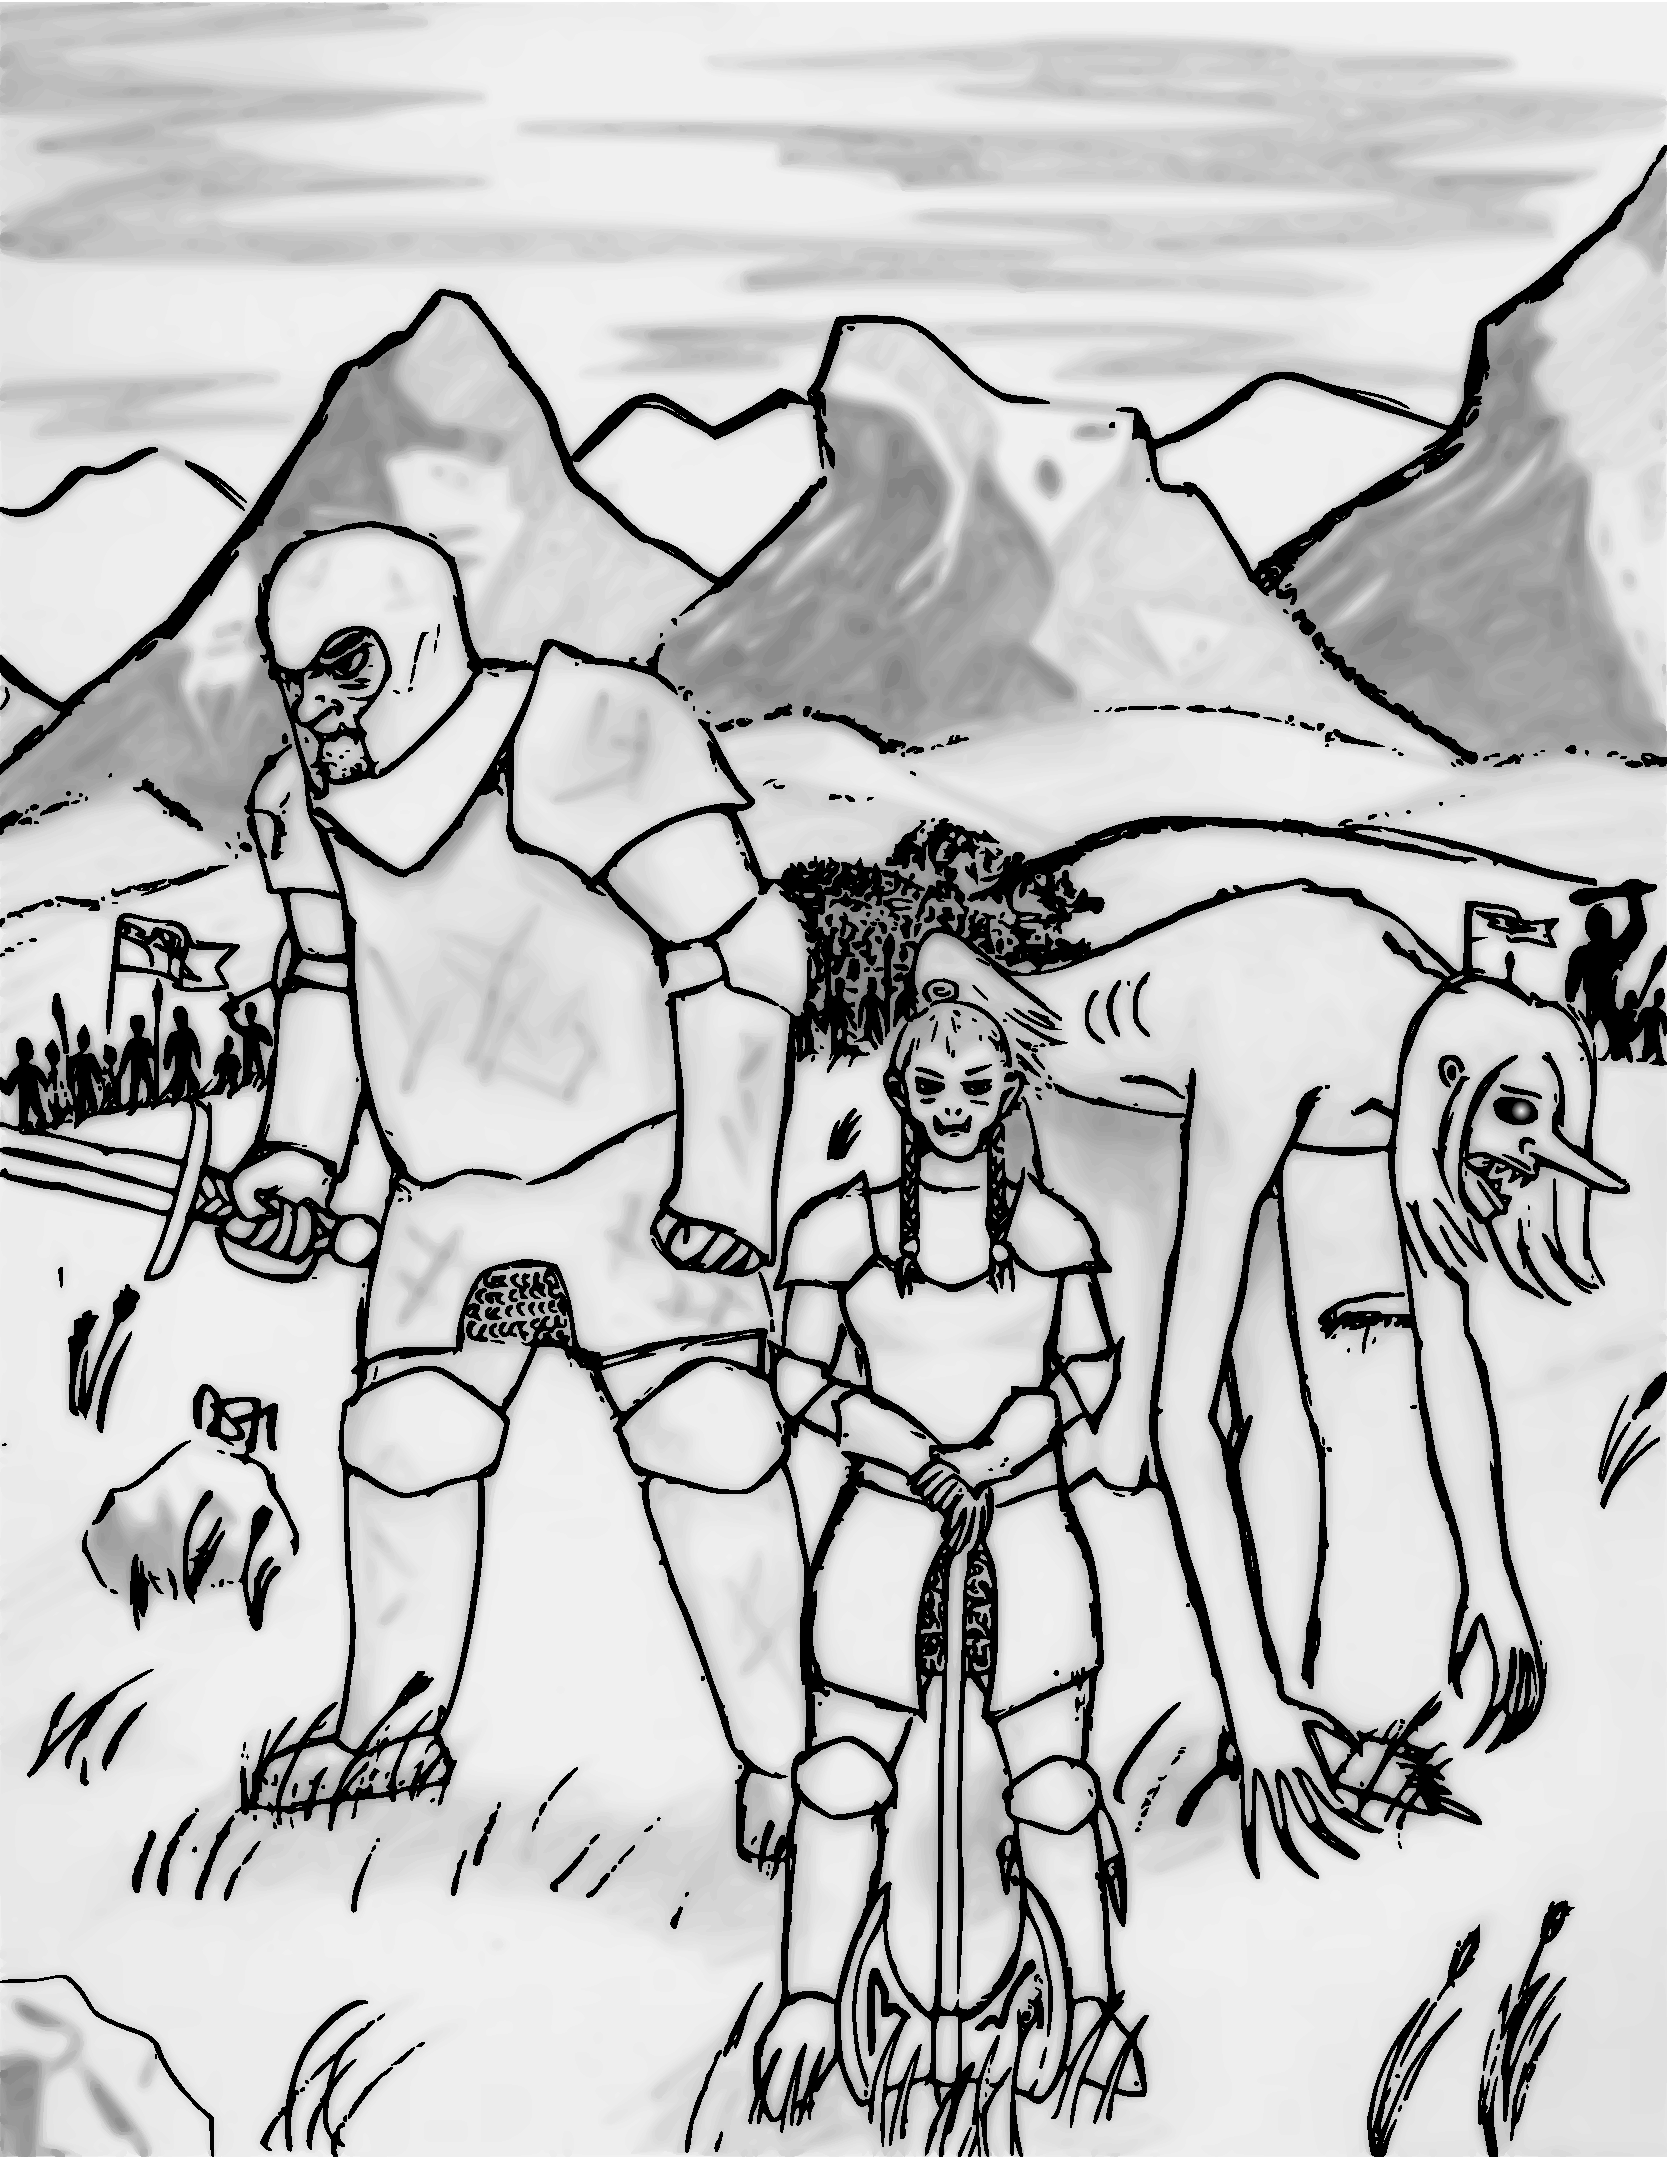
\includepdf[scale=1.007]{gothron.pdf}
